\documentclass[12pt,letterpaper]{article}
\usepackage[utf8]{inputenc}
\usepackage[left=2cm,right=2cm,top=2cm,bottom=2cm]{geometry}
\usepackage{multirow}
\title{Informe Oracle}
\author{Juan Rodriguez}
\date{November 2018}



\usepackage{graphicx}

\begin{document}
    
    \begin{center}
        
\includegraphics[width=4cm]{Imagenes/upt-logo.png}\\
        \vspace{12pt}
        \vspace{12pt}
        \large\textbf{UNIVERSIDAD PRIVADA DE TACNA}\\
        \vspace{12pt}
        \vspace{12pt}
        \large{FACULTAD DE INGENIERÍA}\\
        \vspace{12pt}
        \vspace{12pt}
        \large{Escuela Profesional de Ingeniería de Sistemas}\\
        \vspace{12pt}
        \vspace{12pt}
        \textbf{INSTALACIÓN DE WINDOWNS SERVER 2016 Y ORACLE DATABASE}\\
        \vspace{12pt}
        \vspace{12pt}
        Curso: Bases de Datos II\\
        \vspace{12pt}
        Docente: Ing. Patrick Cuadros\\
        \vspace*{12pt}
           \begin{flushleft}
        Alumno:\\
        \vspace{12pt}
        Rodriguez Mamani, Juan Rigoberto\hfill (2017057862)\\

        \end{flushleft}
        \vspace{100pt}

        Tacna – Perú\\
            2018
        \vspace{12pt}

            \thispagestyle{empty} % CARATULA SIN NUMERO
            \newpage
    		\tableofcontents % INDICE
    		\thispagestyle{empty} % INDICE SIN NUMERO
            \setcounter{page}{1} % REINICIAR CONTADOR DE PAGINAS
    \end{center}
    \break
    
    
\section{Introduccion}
\vspace{12pt}

Oracle es básicamente una herramienta cliente/servidor para la gestión de base de datos, es un producto vendido a nivel mundial, aunque la gran potencia que tiene y su elevado precio hace que solo se vea en empresas muy grandes y multinacionales, por norma general.
\vspace{12pt}\\
En el desarrollo de paginas Web pasa lo mismo como es un sistema muy caro no está tan extendido como otras bases de datos, por ejemplo, Access, MySQL, SQL Server etc.
\vspace{12pt}\\
Oracle como antes lo mencionamos se basa en la tecnología cliente/ servidor, pues bien, para su utilización primero seria necesario la instalación de la herramienta servidor ( Oracle8i ) y posteriormente podríamos atacar a la base de datos desde otros equipos con herramientas de desarrollo como Oracle Designer y Oracle Developer, que son las herramientas de programación sobre Oracle a partir de esta premisa vamos a desarrollar las principales acepciones de Oracle y sus aplicaciones en las distintas ares de trabajo.
\vspace{12pt}\\
Es posible lógicamente atacar a la base de datos a través del SQL plus incorporado en el paquete de programas Oracle para poder realizar consultas, utilizando el lenguaje SQL.
\vspace{12pt}\\
El Developer es una herramienta que nos permite crear formularios en local, es decir, mediante esta herramienta nosotros podemos crear formularios, compilarlos y ejecutarlos, pero si queremos que los otros trabajen sobre este formulario deberemos copiarlo regularmente en una carpeta compartida para todos, de modo que, cuando quieran realizar un cambio, deberán copiarlo de dicha carpeta y luego volverlo a subir a la carpeta.
\vspace{12pt}\\
Este sistema como podemos observar es bastante engorroso y poco fiable pues es bastante normal que las versiones se pierdan y se machaquen con frecuencia. La principal ventaja de esta herramienta es que es bastante intuitiva y dispone de un modo que nos permite componer el formulario, tal y como lo haríamos en Visual Basic o en Visual C, esto es muy de agradecer.

\section{Objetivos}
\vspace{12pt}

-Poner en practica los conocimientos necesarios para realizar la Instalación de un servidor de Base de Datos Oracle sobre un sistema operativo Linux.\\
-Realizar la Instalación de Windows Server 2016.\\
-Realizar de forma correcta la instalación de la Base de Datos Oracle dentro de un ambiente virtualizado.\\
\section{Marco Teórico}
\vspace{12pt}

\subsection{Definición}
Oracle Database es un sistema de gestión de base de datos de tipo objeto-relacional (ORDBMS, por el acrónimo en inglés de Object-Relational Data Base Management System), desarrollado por Oracle Corporation.\\
Su dominio en el mercado de servidores empresariales había sido casi total hasta que recientemente tiene la competencia del Microsoft SQL Server y de la oferta de otros RDBMS con licencia libre como PostgreSQL, MySQL o Firebird.\\
Las últimas versiones de Oracle han sido certificadas para poder trabajar bajo GNU/Linux.\\


\subsection{Historia}

Oracle surge en 1977 bajo el nombre de SDL (Software Development Laboratories).
En 1979, SDL cambia su nombre por Relational Software, Inc. (RSI).
La fundación de SDL fue motivada principalmente a partir de un estudio sobre los SGBD (Sistemas Gestores de Base de Datos) de George Koch. Computer World definió este estudio como uno de los más completos jamás escritos sobre bases de datos. Este artículo incluía una comparativa de productos que dirigía a Relational Software como el más completo desde el punto de vista técnico. 
La tecnología Oracle se encuentra prácticamente en todas las industrias alrededor del mundo y en las oficinas de 98 de las 100 empresas Fortune 100. Oracle es la primera compañía de software que desarrolla e implementa software para empresas cien por ciento activado por Internet a través de toda su línea de productos: base de datos, aplicaciones comerciales y herramientas de desarrollo de aplicaciones y soporte de decisiones. Oracle es el proveedor mundial líder de software para administración de información, y la segunda empresa de software.
\vspace{12pt}\\
\textbf {Oracle, a partir de la versión 10g Release 2, cuenta con 7 ediciones:}\\
Enterprise Edition (EE).\\
Standard Edition (SE).\\
Standard Edition One (SE1).\\
Standard Edition 2 (SE2).\\
Express Edition (XE).\\
Personal Edition (PE).\\
Lite Edition (LE).\\
\vspace{12pt}\\

\section{Desarrollo}

\subsection{PARTE I: Instalación Hyper-V}

\textbf {4.1.1. Verificar Edición de Windows 10:} El Hyper V es una característica de Windows 10 en las versiones PRO y Educational, para esto primero verificaremos si nuestro sistema pertenece a alguna de esas ediciones.
\begin{center}
  
\includegraphics[width=15cm]{Imagenes/Windows_Education.png}
\end{center}

\textbf {4.1.2. Buscar la opción de Características de Windows:} Nos dirigimos al Menu del Windows 10 y buscamos la opción de "Activar o desactivar las caracterísitcas de Windows".\\
\begin{center}
  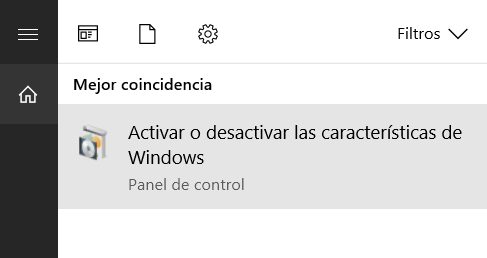
\includegraphics[width=15cm]{Imagenes/Activar_Caracteristicas.png}
\end{center}
\break

\textbf {4.1.3. Activar Característica Hyper-V:} Buscamos la opción llamada "Hyper V" y lo activamos.\\
\begin{center}
  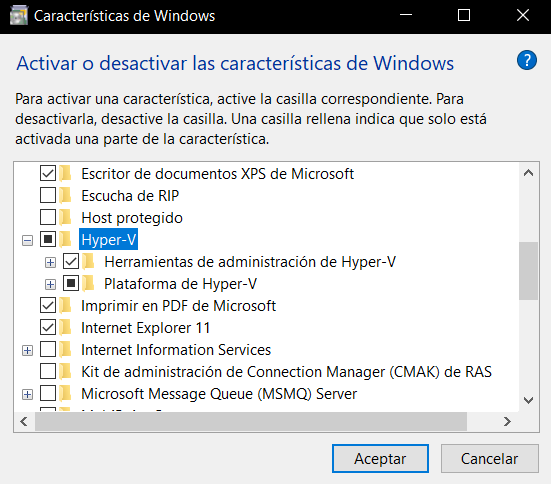
\includegraphics[width=11cm]{Imagenes/Activar_Hyper_V.png}
\end{center}

\textbf {4.1.4. Reiniciar el Sistema Operativo:} Con la finalidad de que se apliquen los cambios, es necesario reiniciar el equipo.
\begin{center}
  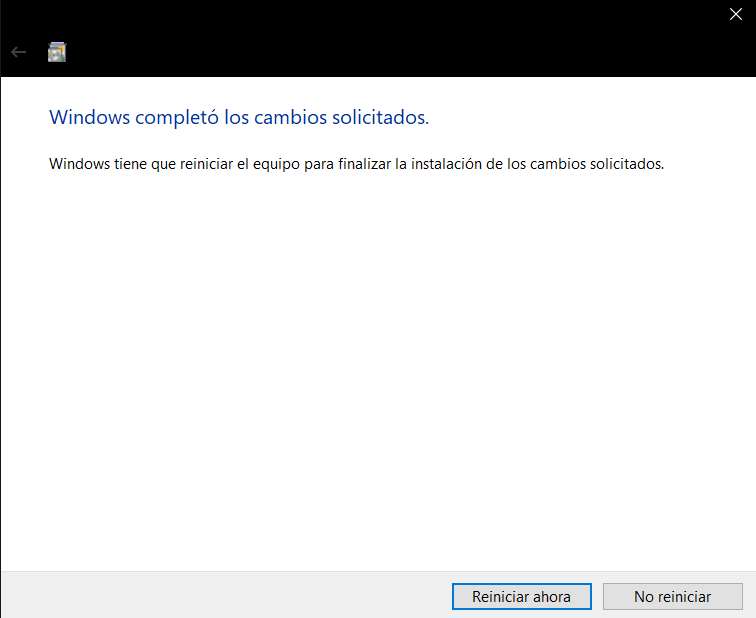
\includegraphics[width=11cm]{Imagenes/Reiniciar.png}
\end{center}
\break

\textbf {4.1.5. Hyper V correctamente habilitado:} Una vez reiniciada la computadora, ya podremos abrir nuestro Hyper-V que estará listo para ser configurada.\\
\begin{center}
  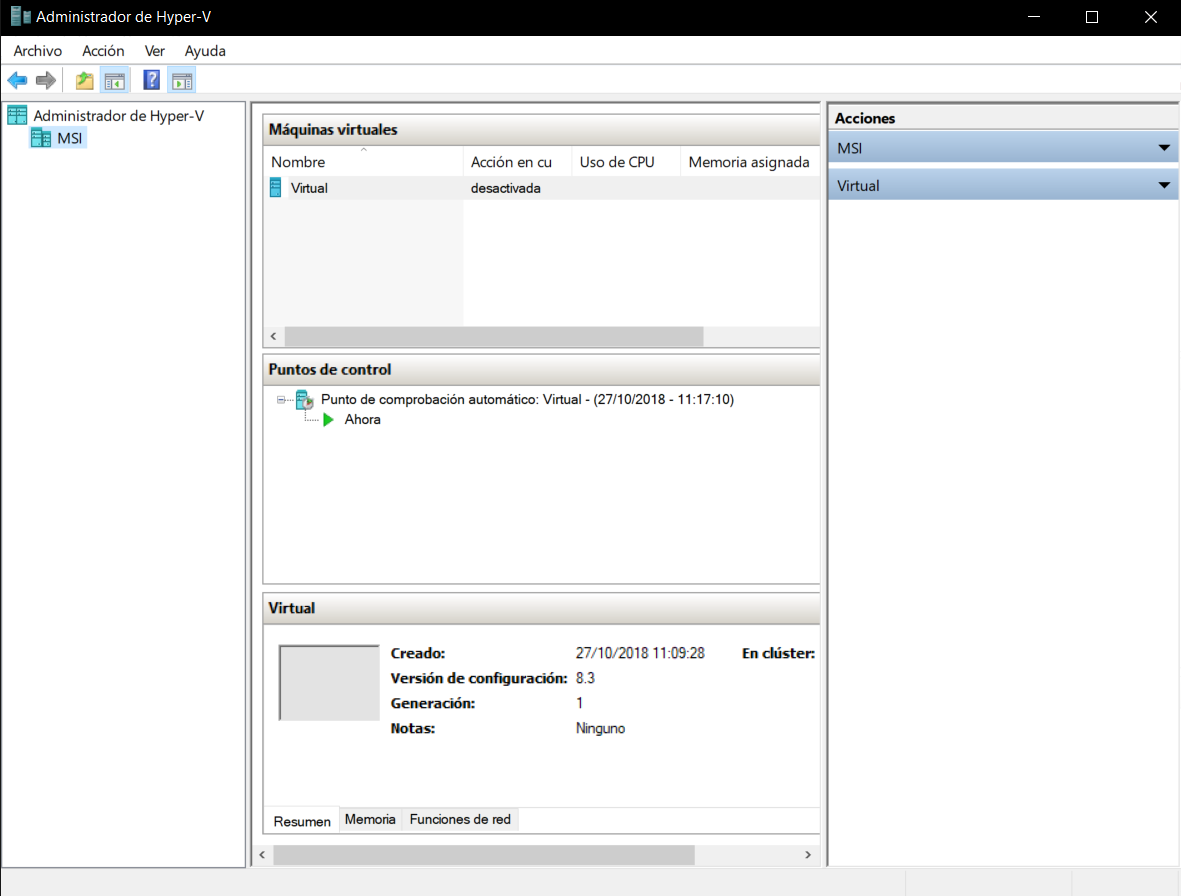
\includegraphics[width=14cm]{Imagenes/Hyper_V.png}
\end{center}
\break

\subsection{PARTE II: Instalación Windows Server 2016}

\textbf {4.2.1. Crear Nueva maquina Virtual:} En este paso crearemos una nueva maquina virtual donde instalaremos nuestro Windows Server 2016, para eso le daremos clic derecho a nuestro servidor de HYPER V.
\begin{center}
  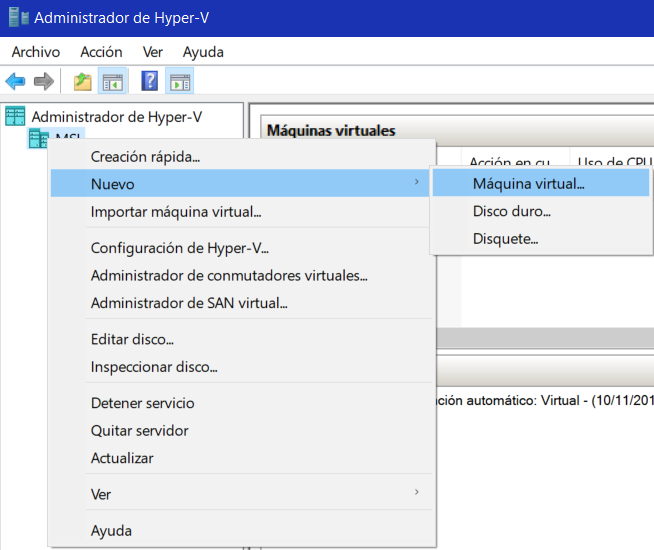
\includegraphics[width=11cm]{Imagenes/Nueva_Maquina.png}
\end{center}

\textbf {4.2.2. Especificar Nombre:} Ahora especificaremos el nombre de nuestra maquina virtual, en este caso le colocaremos Windows Server 2016.
\begin{center}
  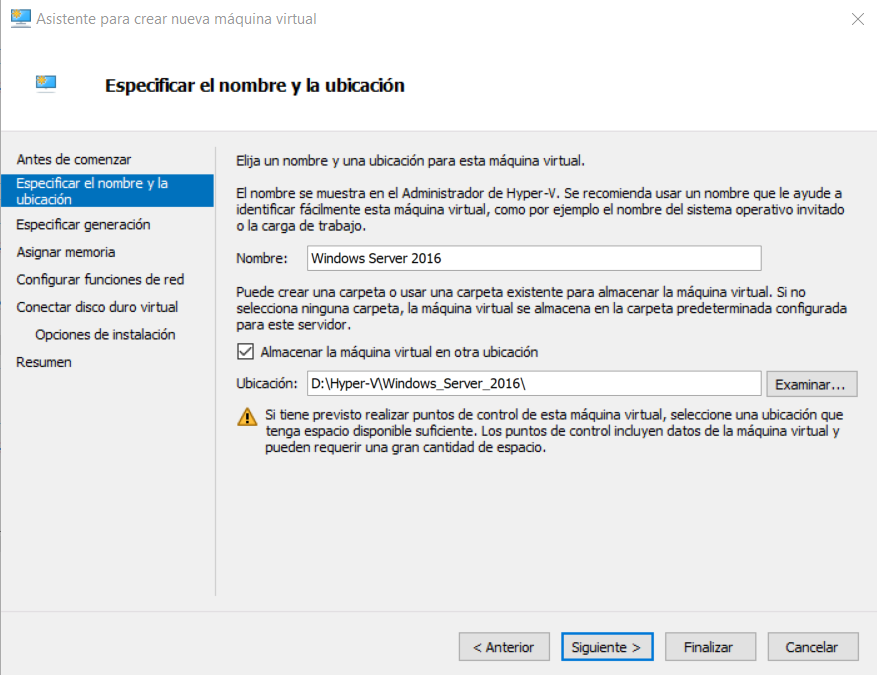
\includegraphics[width=11cm]{Imagenes/Especificar_Nombre_Ruta.png}
\end{center}
\break

\textbf {4.2.3. Elegir Generación:} Elegiremos la Generación que se marca por defecto, en este caso es la Generación 1.
\begin{center}
  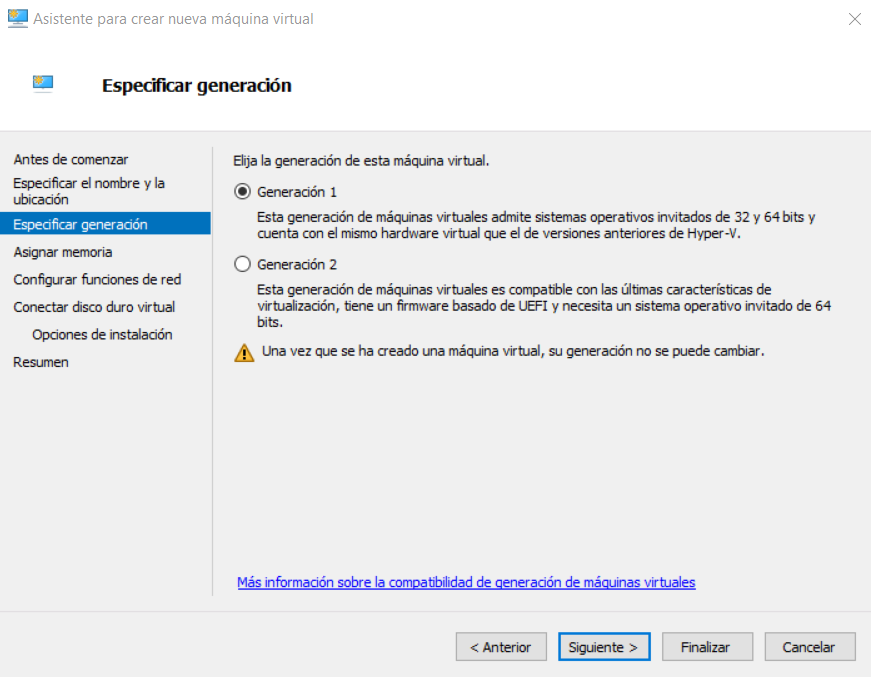
\includegraphics[width=11cm]{Imagenes/Especificar_Generacion.png}
\end{center}

\textbf {4.2.4. Asignar Memoria:} Elegiremos la cantidad de memoria con la que queremos que trabaje nuestra maquina virtual, en este caso le pusimos 2048mb y le damos clic en Siguiente.
\begin{center}
  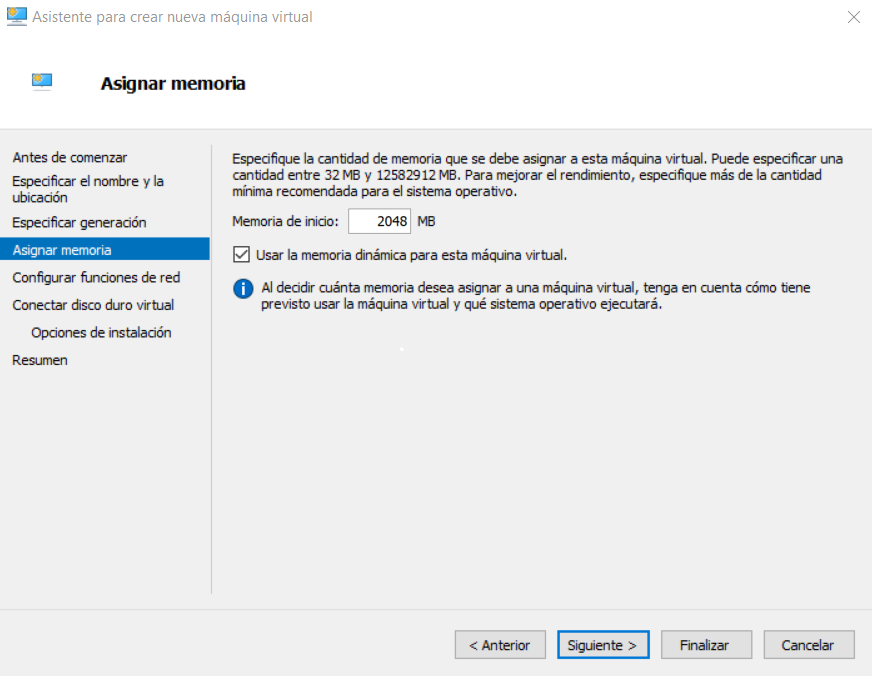
\includegraphics[width=11cm]{Imagenes/Asignar_Memoria.png}
\end{center}
\break

\textbf {4.2.5. Conectar Disco:} Estableceremos la ruta de nuestra maquina virtual y le asignaremos el tamaño de 80GB.
\begin{center}
  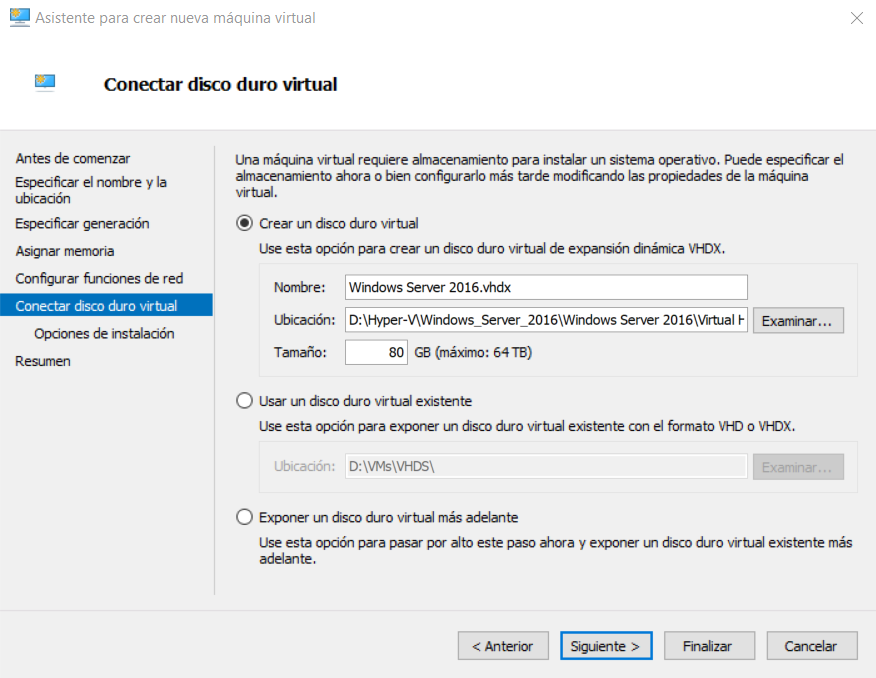
\includegraphics[width=11cm]{Imagenes/Conectar_Disco.png}
\end{center}

\textbf {4.2.6. Resumen:} Al terminar con la configuración, el asistente nos mostrará un Resumen de nuestra máquina virtual, si todo esta conforme le daremos clic en FINALIZAR.
\begin{center}
  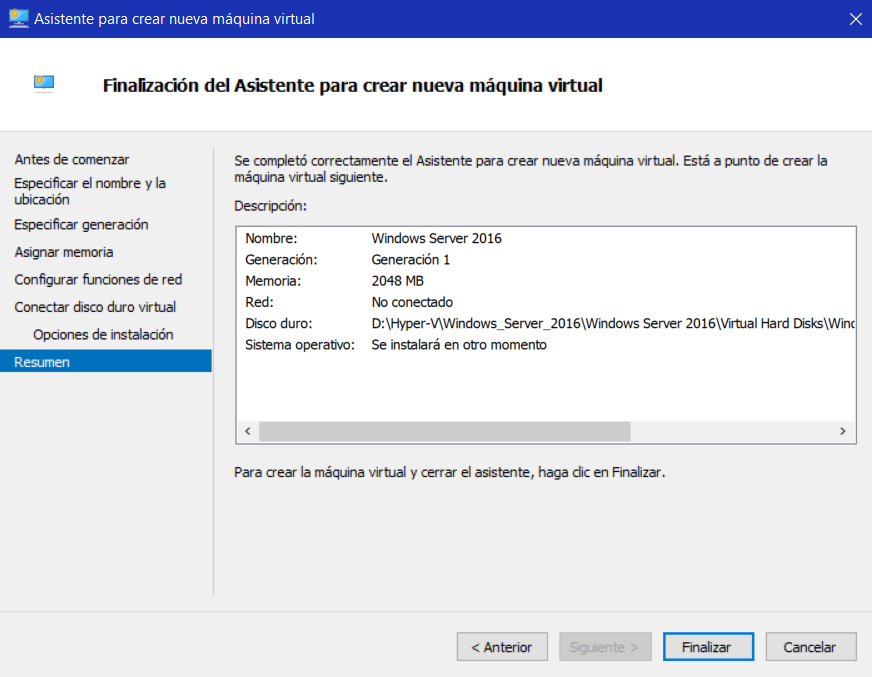
\includegraphics[width=11cm]{Imagenes/Resumen.png}
\end{center}
\break

\textbf {4.2.7. Conectar con la Máquina Virtual:}Para este paso le daremos clic derecho sobre nuestra máquina virtual y le damos clic en Conectar.
\begin{center}
  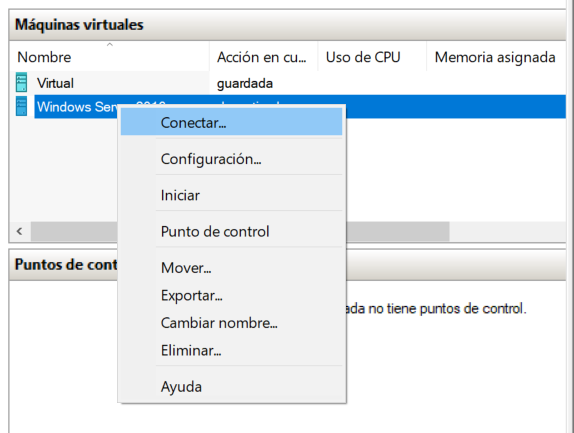
\includegraphics[width=11cm]{Imagenes/Conectar_WindowsServer.png}
\end{center}

\textbf {4.2.8. Iniciar Virtualización:} Una vez que hayamos conectado nuestra máquina virtual, se nos abrirá el virtualizador, nosotros le daremos clic en INICIAR, para que comience a virtualizar.
\begin{center}
  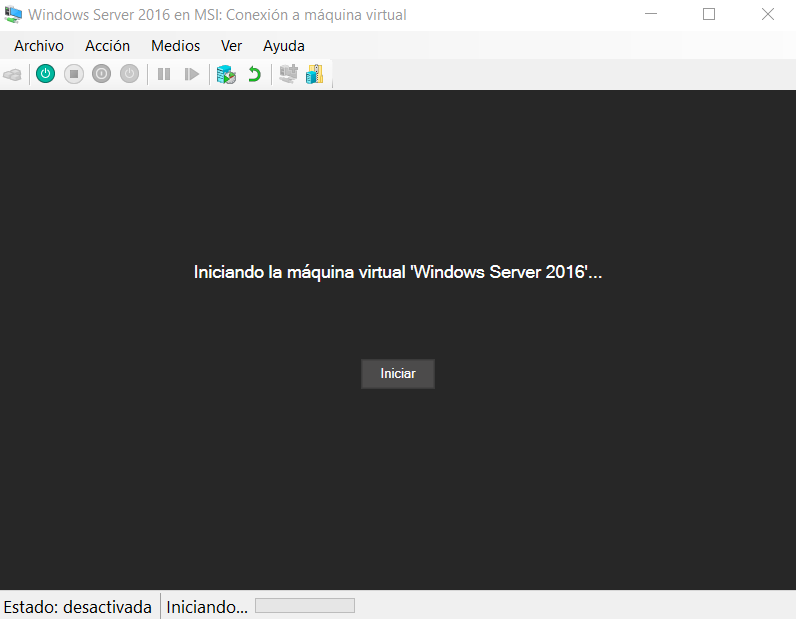
\includegraphics[width=11cm]{Imagenes/Iniciar_Virtualizacion.png}
\end{center}
\break

\textbf {4.2.9. Elegir el ISO de instalación:}Para este paso le daremos clic en Medios - Unidad de DVD y seleccionaremos la nuestro ISO.
\begin{center}
  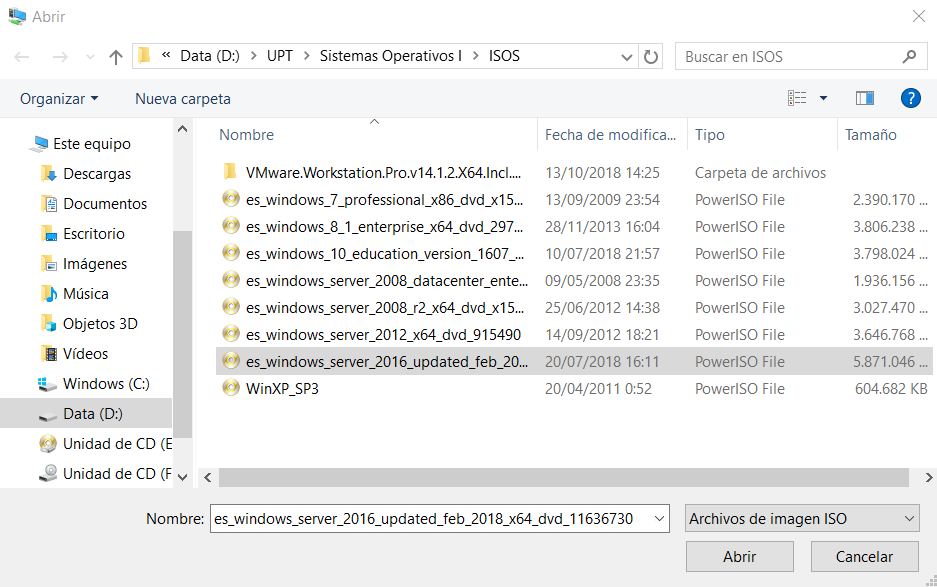
\includegraphics[width=11cm]{Imagenes/Elegir_ISO.png}
\end{center}

\textbf {4.2.10. Iniciar Instalación:} Luego de elegir nuestro ISO, volveremos a Iniciar nuestra Virtualización seguidamente nos aparecerá el cuadro de Instalación de Windows Server.
\begin{center}
  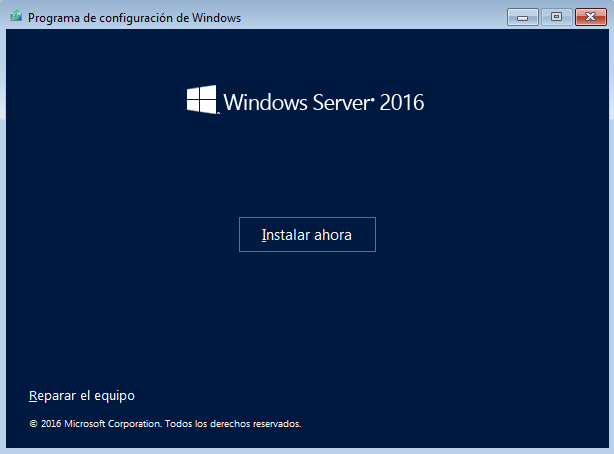
\includegraphics[width=11cm]{Imagenes/Instalar_Ahora.png}
\end{center}
\break

\textbf {4.2.11. Configuración de la Instalación:} Luego de hacer clic en Instalar Ahora, nos aparecera un cuadro donde podremos elegir el tipo de Idioma que deseamos usar en nuestro Windows Server, nosotros elegiremos Español Perú y le daremos clic en Siguiente.
\begin{center}
  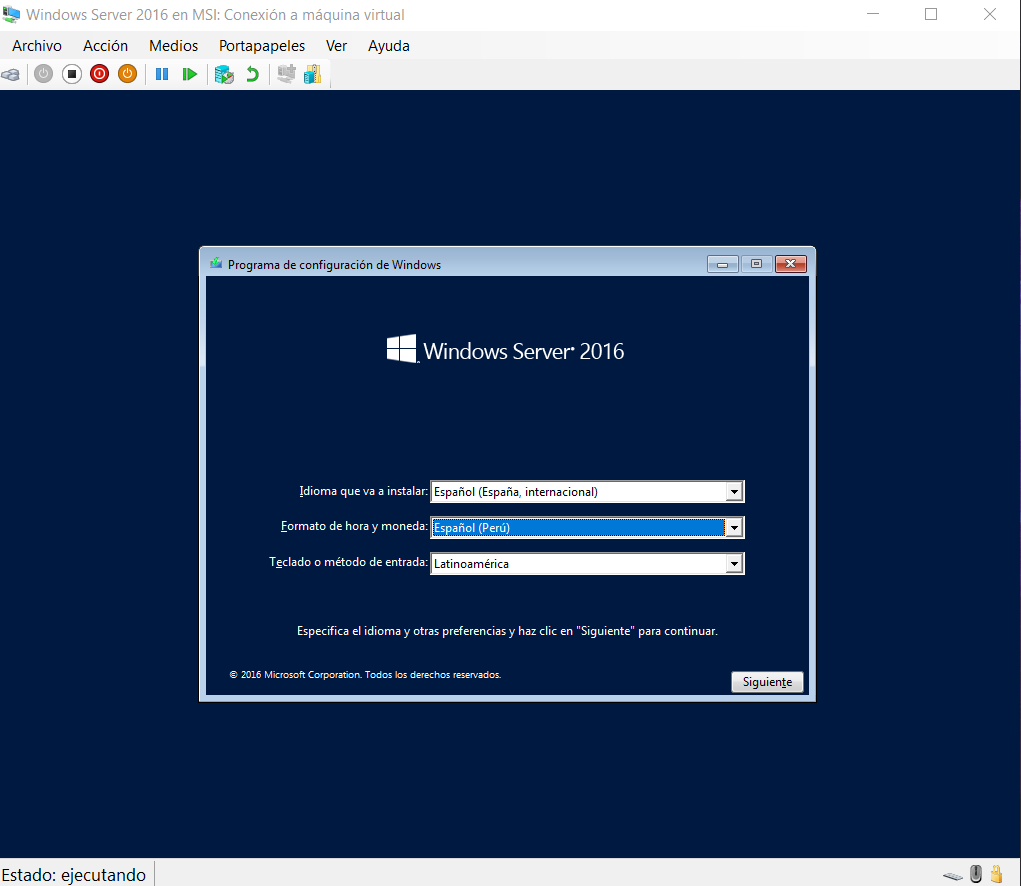
\includegraphics[width=11cm]{Imagenes/Iniciar_Instalacion.png}
\end{center}

\textbf {4.2.12. Ingresar Serial:} Si hemos comprado el software, debemos ingresar el Serial que llega junto al Instalador, en caso de no tener el Serial le damos clic en la opción: No tengo Clave del Producto y Siguiente.
\begin{center}
  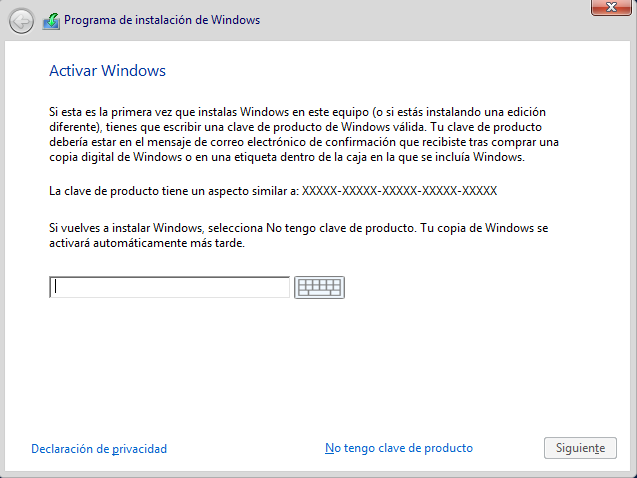
\includegraphics[width=11cm]{Imagenes/Ingresar_Serial.png}
\end{center}
\break

\textbf {4.2.13. Elegir Versión:} Elegiremos la opción de Windows Server 2016 DataCenter (Experiencia de Escritorio) y le damos clic en Siguiente
\begin{center}
  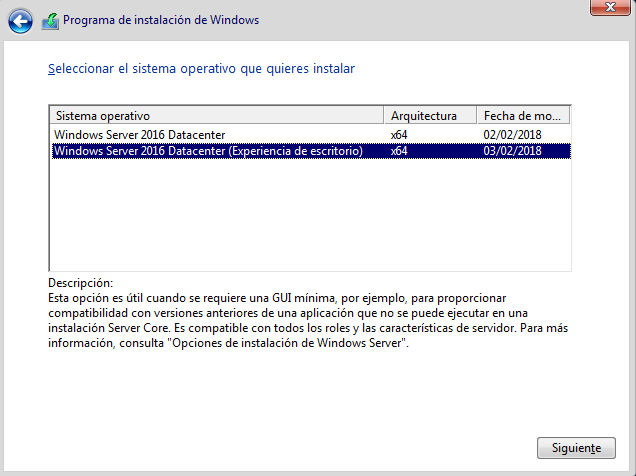
\includegraphics[width=11cm]{Imagenes/Elegir_Version.png}
\end{center}

\textbf {4.2.14. Aceptar Licencia:} Leeremos los términos y licencia y activaremos el check de ACEPTO, y luego clic en Siguiente.
\begin{center}
  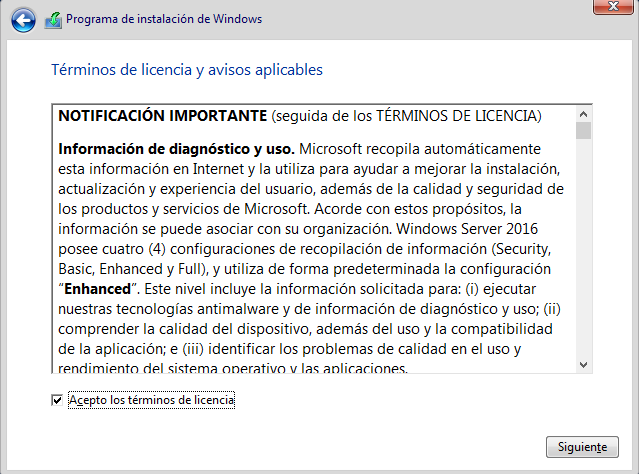
\includegraphics[width=11cm]{Imagenes/Aceptar_Licencia.png}
\end{center}
\break

\textbf {4.2.15. Tipo de Instalación:} Nosotros le daremos clic en Instalación Personalizada.
\begin{center}
  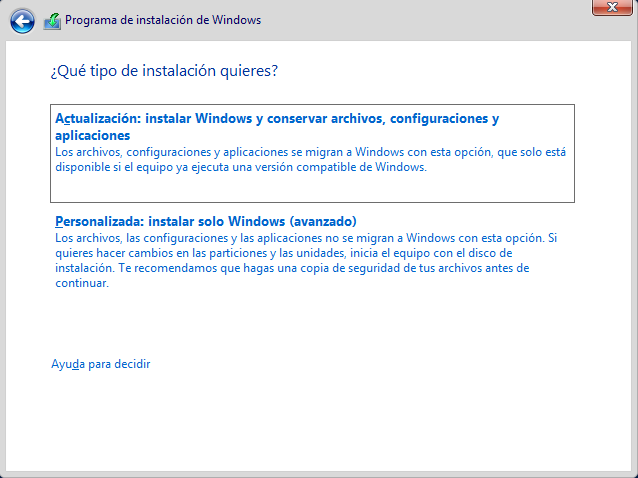
\includegraphics[width=11cm]{Imagenes/Elegir_Tipo_Instalacion.png}
\end{center}

\textbf {4.2.16. Disco de Instalación:} Elegiremos el único disco disponible (Unidad 0) y le daremos clic en Siguiente.
\begin{center}
  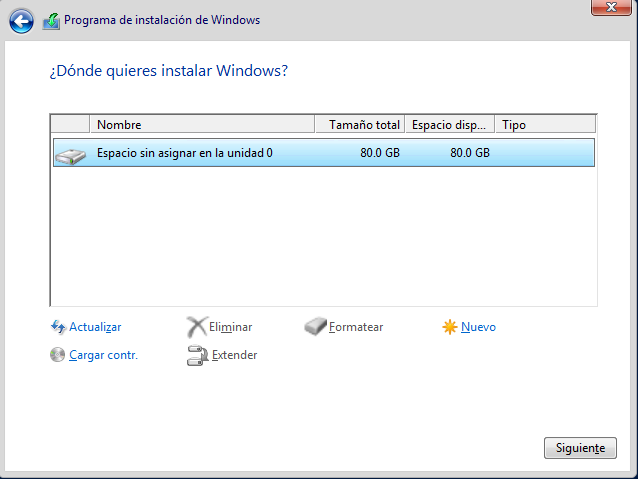
\includegraphics[width=11cm]{Imagenes/Elegir_Disco_Instalacion.png}
\end{center}
\break

\textbf {4.2.17. Proceso de Instalacion:} Luego comenzará la Instalación de nuestro Windows Server, en este paso solo queda esperar a que la Instalación termine.
\begin{center}
  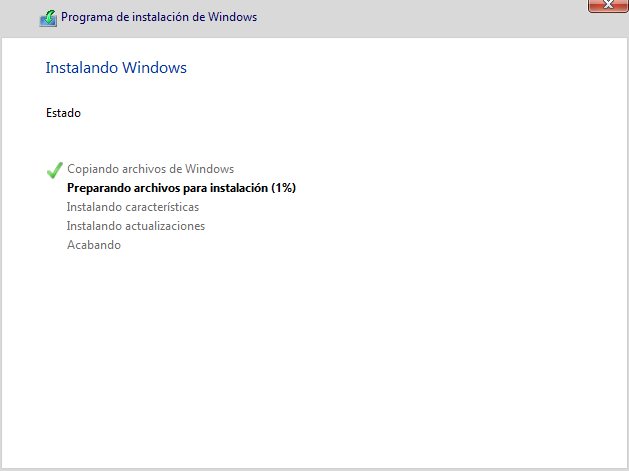
\includegraphics[width=11cm]{Imagenes/Proceso_Instalacion.png}
\end{center}

\textbf {4.2.18. Crear Clave:} Luego de que el Proceso de Instalación haya terminado, ahora debemos crear una clave para el Administrador del Servidor, en este caso nosotros le asignaremos la clave de: Sistemas.2018
\begin{center}
  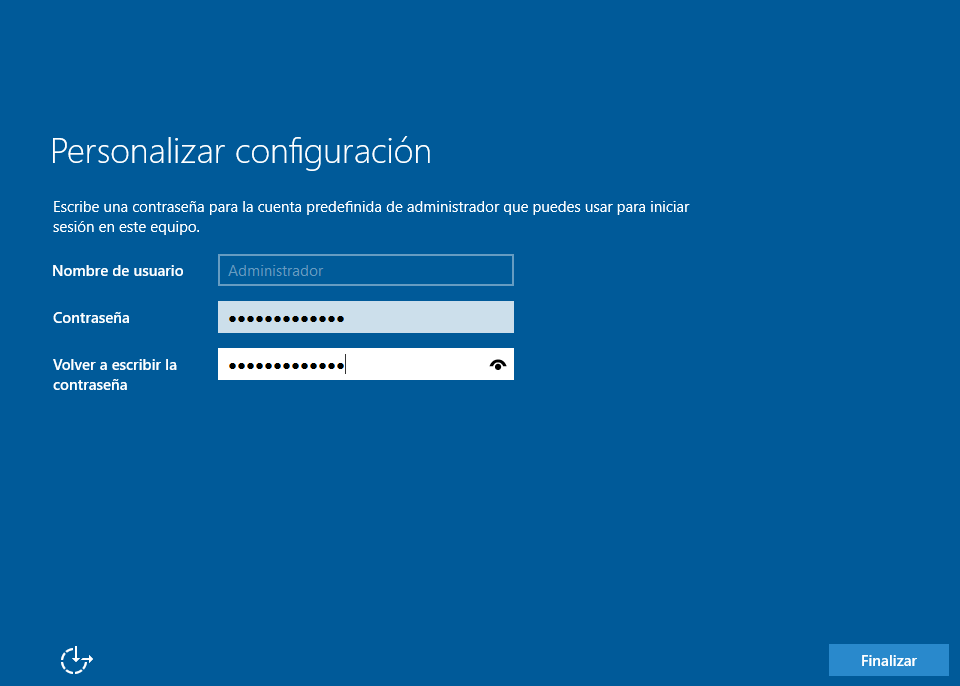
\includegraphics[width=11cm]{Imagenes/Crear_Clave.png}
\end{center}
\break

\textbf {4.2.19. Identificarse en el Windows Server:} En este paso debemos identificarnos para poder iniciar nuestro Windows Server, para esto ingresaremos con la contraseña antes creada: Sistemas.2018
\begin{center}
  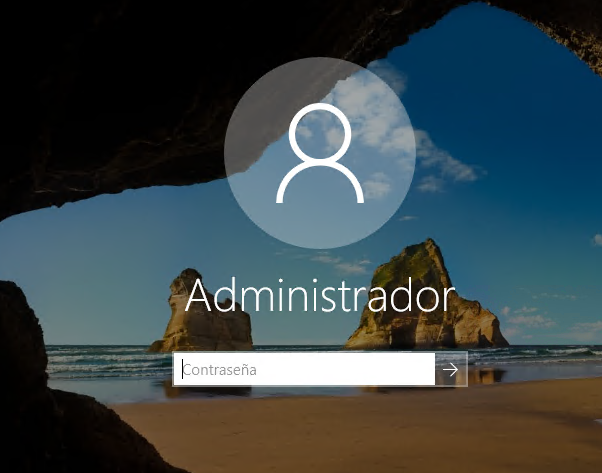
\includegraphics[width=11cm]{Imagenes/Identificarse.png}
\end{center}

\textbf {4.2.20. Windows Server 2016:} Luego de tanta espera, al fin podremos acceder a nuestro Windows Server la cuál se encuentra lista para poder instalarle el Oracle DataBase.
\begin{center}
  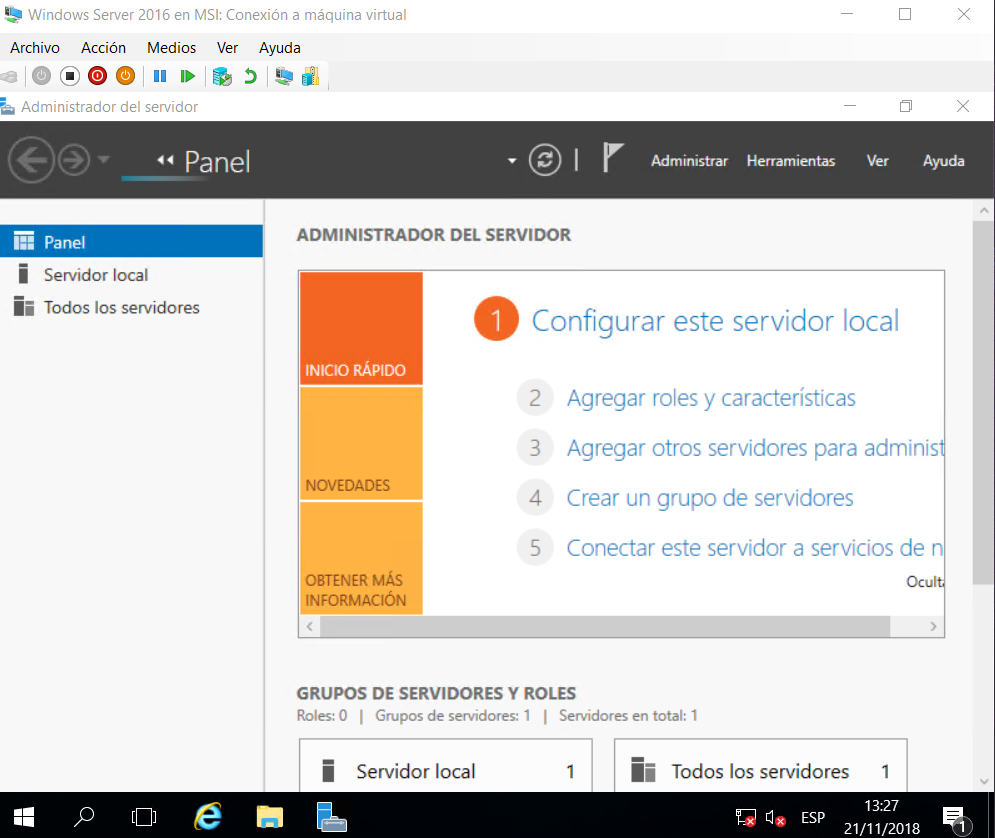
\includegraphics[width=11cm]{Imagenes/Escritorio_Windows_Server.png}
\end{center}
\break
\section{Conclusiones}
\vspace{12pt}

• Oracle es uno de los motores de base de datos relacional más utilizado a nivel mundial.\\
• Puede ejecutarse en todas las plataformas de hardware, desde una laptop, una PC, hasta en un supercomputador.\\
• Oracle soporta todas las funciones que se esperan de un servidor: un lenguaje de diseño de bases de datos muy completo (PL/SQL) que permite implementar diseños "activos", con triggers y procedimientos almacenados, con una integridad referencial declarativa bastante potente.\\
• Permite el uso de particiones para la mejora de la eficiencia, de replicación e incluso ciertas versiones admiten la administración de bases de datos distribuidas.\\
• En cuanto a seguridad, Oracle brinda al usuario un set de funcionalidades para obtener un ambiente muy seguro.\\
\section{Bibliografia}
\begin{thebibliography}{9}
\bibitem{latexcompanion} 
Michel Goossens, Frank Mittelbach, and Alexander Samarin. 
\textit{Oracle Database}. 
Addison-Wesley, Reading, Massachusetts, 2009.
 
\bibitem{einstein} 
Albert Einstein. 
\textit{Zur  bewegter K{\"o}rper}. (German) 
[\textit{Cómo activar y usar el cliente Hyper-V}]. 
Annalen der Physik.
 
\bibitem{knuthwebsite} 
Knuth:  Install Windows server 2016 on Hyper V Tutorial 1, Youtube
\\\texttt{https://www.youtube.com/watch?v=d-JfrrsDq-g/\~{}uno/abcde.html}
\end{thebibliography}
    

\end{document}

